\documentclass[10pt,a4paper]{article}
\usepackage[utf8]{inputenc}
\usepackage[francais]{babel}
\usepackage[T1]{fontenc}
\usepackage{amsmath}
\usepackage{amsfonts}
\usepackage{amssymb}
\usepackage{graphicx}
\usepackage{float}
\usepackage{array}
\usepackage[left=2cm,right=2cm,top=2cm,bottom=2cm]{geometry}
\usepackage[svgnames]{xcolor}
\usepackage{listings}

\lstset{language=python,
	frame=single,
    basicstyle=\small\ttfamily,
    stringstyle=\color{DarkGreen},
    otherkeywords={0,1,2,3,4,5,6,7,8,9},
    morekeywords={TRUE,FALSE},
    deletekeywords={data,frame,length,as,character},
    keywordstyle=\color{blue},
    commentstyle=\color{DarkGreen},
}

\setlength{\parindent}{0pt}

\begin{document}

\author{Guillaume Bernard-Reymond}
\title{TP3 - Support Vector Machine (SVM)}
\maketitle

Le but de ce TP est de mettre en pratique ce type de techniques de classification sur données réelles et
simulées au moyen du package scikit-learn (lequel met en \oe uvre la librairie en C libsvm) et d'apprendre
à contrôler les paramètres garantissant leur flexibilité (hyper-paramètres, noyau)

\medskip

Dans tout le rapport, les résultats seront arrondis à $10^{-4}$ pour garder une certaine précision tout en restant lisible. On trouvera tout au long du compte-rendu les morceaux de code qui étaient à compléter ainsi que des ajouts personnels.

\medskip

\begin{large}
\textbf{Première mise en \oe uvre}
\end{large}

\textbf{Question 1 et 2 :}

On sépare d'abord le jeu de données \texttt{iris} en deux parties : une pour l'entrainement et l'autre pour le test : 

\begin{lstlisting}
X, y = shuffle(X, y)
X_train, X_test, y_train, y_test = train_test_split(X, y, train_size=0.5)
\end{lstlisting}

J'ai dans un premier temps appliquer une SVM au jeu de données \texttt{iris} sans optimisation du choix des paramètres par l'utilisation de la fonction \texttt{GridSearchCV} dans le cas linéaire et polynomiale : 

\begin{table}[H]
% \usepackage{array} is required
\begin{center}
 \begin{tabular}{|l|>{\centering\arraybackslash}p{2cm}|}
\hline 
\rule[-1ex]{0pt}{2.5ex} Noyau linéaire & 0.56 \\ 
\hline 
\rule[-1ex]{0pt}{2.5ex} Noyau polynomiale & 0.5 \\ 
\hline 
\end{tabular}
 \end{center} 
\caption{Comparaison des scores sur la prédiction des classes 1 et 2 du jeu de données iris sans optimisation}
\end{table}

On remarque donc que le choix par défaut du noyau polynomial ne rend pas meilleur la prédiction bien que l'espace de plongement soit supérieur

\medskip

On peut observer aussi le choix de classification qui a été fait : 

\begin{figure}[H]
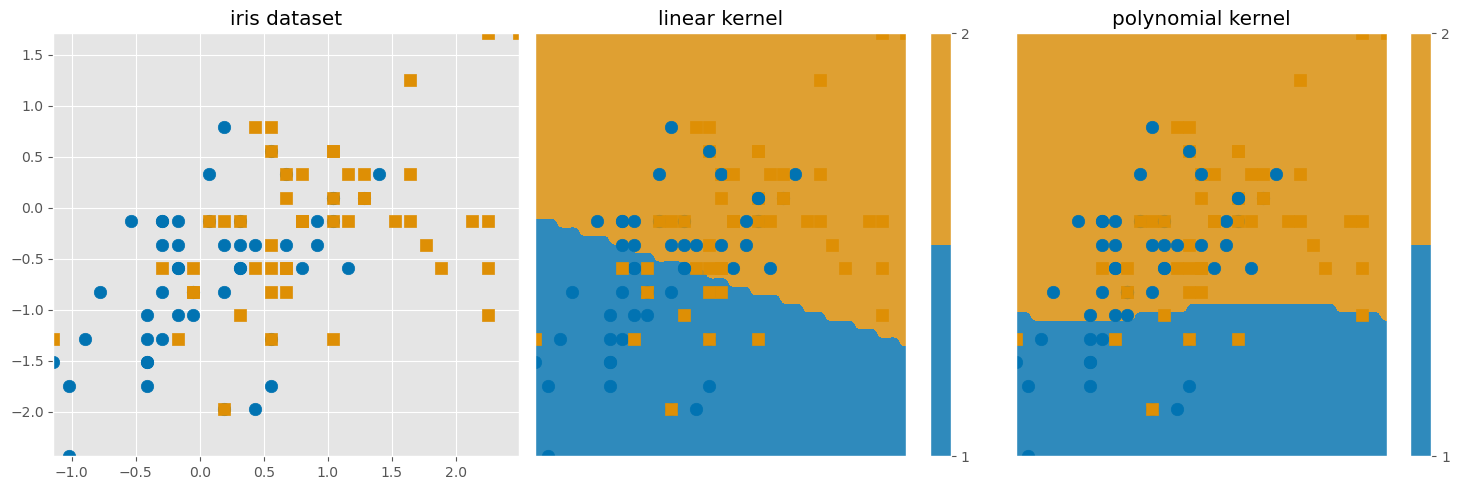
\includegraphics[width=\linewidth]{images/linear_vs_poly_noptim.png}
\caption{Comparaison de la classification des iris entre un noyau linéaire et un noyau polynomial avec paramètres par défaut.}
\label{fig:lin_vs_pol_nopt}
\end{figure}

Maintenant si l'on choisit d'optimiser les paramètres, on obtient à partir du code ci-dessous les résultats suivants : 

\begin{lstlisting}
# fit the model
parameters = {'kernel': ['linear'], 'C': list(np.logspace(-3, 3, 200))}
clf_linear = SVC()
clf_linear_grid = GridSearchCV(clf_linear, parameters, n_jobs=-1)
clf_linear_grid.fit(X_train,y_train)

#calcul de y_pred mais pas forcement utile ici
y_pred=clf_linear_grid.predict(X_test)

# compute the score
print(clf_linear_grid.best_params_)
score = clf_linear_grid.score(X_test,y_test)
\end{lstlisting}

\begin{table}[H]
% \usepackage{array} is required
\begin{center}
 \begin{tabular}{|l|>{\centering\arraybackslash}p{2cm}|}
\hline 
\rule[-1ex]{0pt}{2.5ex} Noyau linéaire & 0.56 \\ 
\hline 
\rule[-1ex]{0pt}{2.5ex} Noyau polynomial & 0.62 \\ 
\hline 
\end{tabular}
 \end{center} 
\caption{Comparaison des scores sur la prédiction des classes 1 et 2 du jeu de données iris avec optimisation}
\end{table}

Le gain d'environ 10,7\% par rapport au noyau linéaire n'est pas négligeable, toutefois il faut prendre les temps de calcul qui sont alors plus long car plus de paramètres sont à tester et à valider. 

\medskip

On observe une classification cette fois ci bien différente :

\begin{figure}[H]
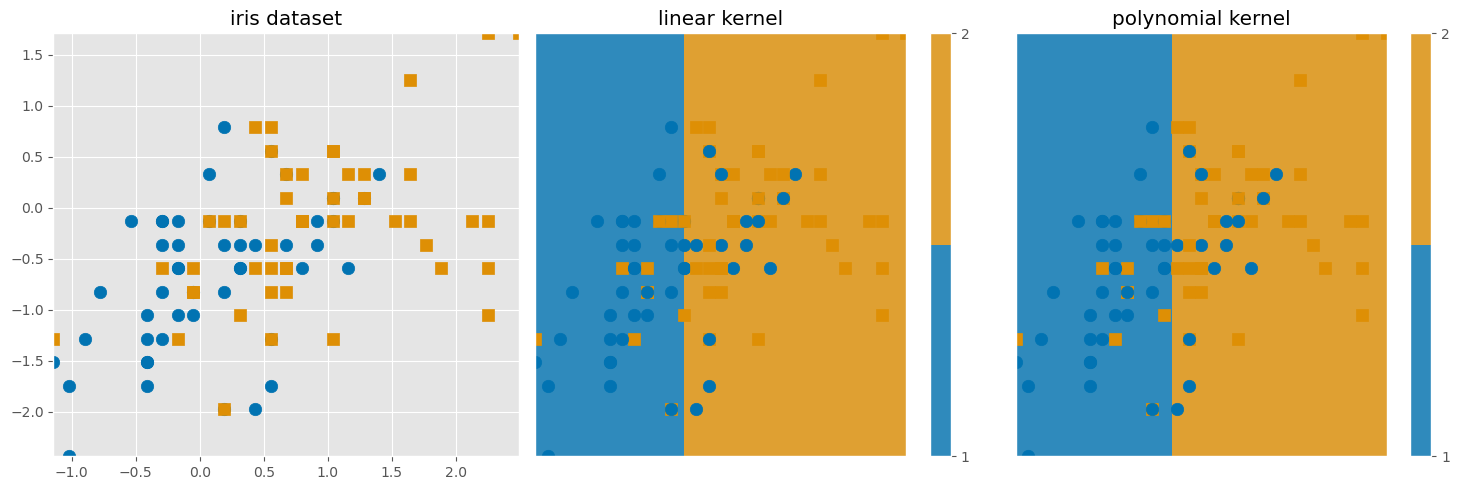
\includegraphics[width=\linewidth]{images/linear_vs_poly_optim.png}
\caption{Comparaison de la classification des iris entre un noyau linéaire et un noyau polynomial optimisé.}
\label{fig:lin_vs_pol_opt}
\end{figure}

Dans notre cas, il semble que pour le noyau polynomiale optimisé, un choix linéaire ait été fait.

\begin{large}
\textbf{SVM GUI}
\end{large}

\textbf{Question 3 :}

Pour un nuage de points fixé dans des proportions 90\% - 10\%, nous nous intéressons à l'influence d'un paramètre $C$ appelé  "constante de tolérance" et qu'il s'agit d'ajuster pour avoir le pourcentage de classement correct le plus élevé : l'accuracy.

\begin{table}[H]
\begin{tabular}{|l|*{6}{>{\centering\arraybackslash}p{2cm}|}}
\hline 
\rule[-1ex]{0pt}{2.5ex} Valeur de $C$ & 1 & 0.1 & 0.01 & 0.001 & 0.0001 & 0.00001 \\ 
\hline 
\rule[-1ex]{0pt}{2.5ex} Accuracy & 96 & 96 & 96 & 92 & 90 & 90 \\ 
\hline 
\end{tabular}
\caption{Evolution de l'accuracy en fonction de la valeur de $C$}
\label{tab:accuracy_vs_C}
\end{table}

\begin{figure}[H]
\begin{tabular}{ccc}
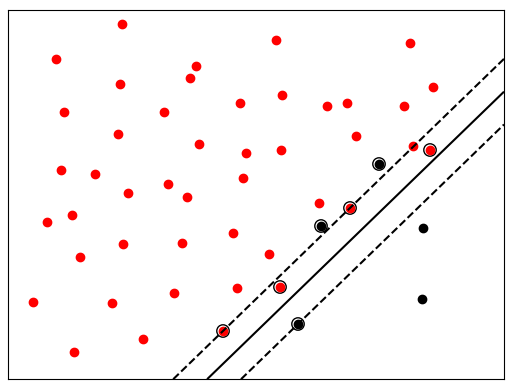
\includegraphics[width=0.33\linewidth]{images/libC1.png} & 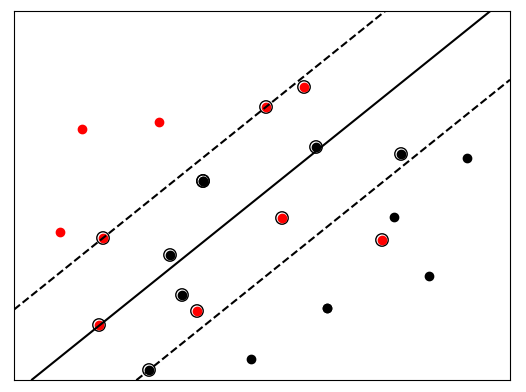
\includegraphics[width=0.33\linewidth]{images/libC0_1.png} & 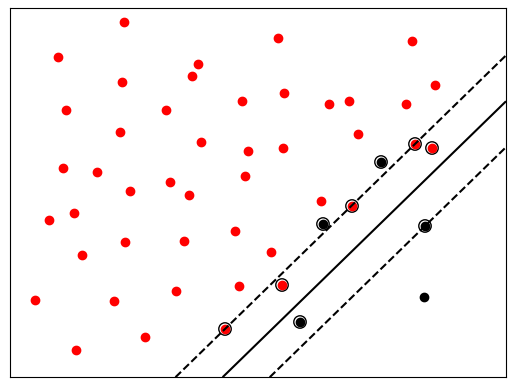
\includegraphics[width=0.33\linewidth]{images/libC0_01.png} \\ 

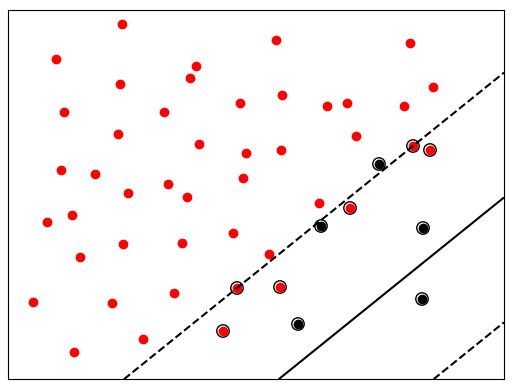
\includegraphics[width=0.33\linewidth]{images/libC0_001.png} & 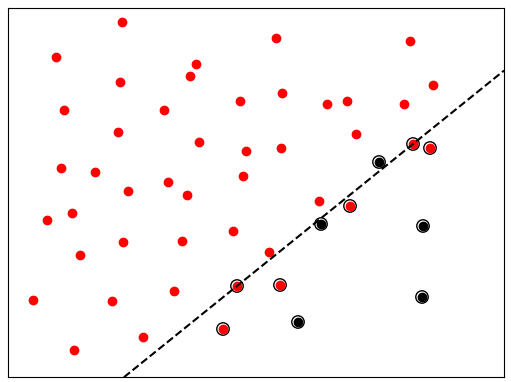
\includegraphics[width=0.33\linewidth]{images/libC0_0001.png} & 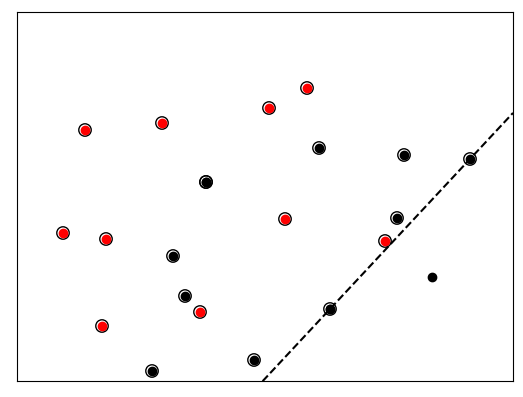
\includegraphics[width=0.33\linewidth]{images/libC0_00001.png} \\ 
\end{tabular} 
\caption{Classification avec un noyau linéaire pour différentes valeurs de C = 1; 0.1 ; 0.01 ; 0.001 ; 0.0001 ; 0.00001 de gauche à droite et de haut en bas}
\end{figure}

On remarque l'accuracy baisse avec la valeur de $C$. Ceci est tout à fait normal car lorsque $C$ diminue, la marge augmente et le pourcentage de bien classé diminue vu qu'on autorise certains à être dans la marge. D'ailleurs pour $C<0,001$, tous les points noirs sont mal classés.
\bigskip

\begin{large}
\textbf{Classification de visages}
\end{large}


\textbf{Question 4 :}

Le score d'apprentissage augmente avec la valeur de $C$ jusqu'à atteindre un palier à partir de $C=10^{-3}$ que l'on va donc considérer comme notre meilleur paramètre.

\begin{lstlisting}
# fit a classifier (linear) and test all the Cs
Cs = 10. ** np.arange(-5, 6)
scores = []
for C in Cs:
    clf = SVC(kernel='linear', C=C)
    clf.fit(X_train, y_train)
    scores.append(clf.score(X_train, y_train))
\end{lstlisting}

\begin{figure}[H]
\centerline{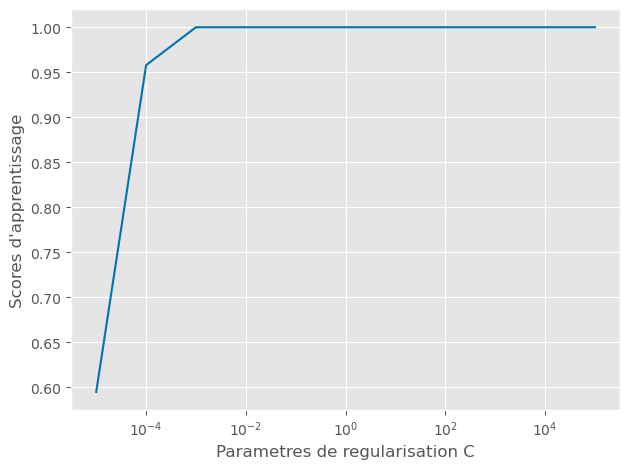
\includegraphics[width=0.6\linewidth]{images/score_vs_C.png}}
\caption{Evolution du score en fonction du paramètre de régularisation C}
\label{fig:sc_vs_c}
\end{figure}

On obtient alors les résultats suivants pour la valeur de $C=10^{-3}$ : 

\begin{itemize}
\item[$\bullet$] Chance level : 0.6211
\item[$\bullet$] Accuracy : 0.9105
\end{itemize}

\begin{lstlisting}
# predict labels for the X_test images with the best classifier
clf = SVC(kernel='linear', C=Cs[ind])
clf.fit(X_train, y_train)
y_pred=clf.predict(X_test)
\end{lstlisting}

\medskip

On pourrait aussi tracer la courbe de l'erreur par validation croisée sur le paramètre $C$.  

\begin{figure}[H]
\centerline{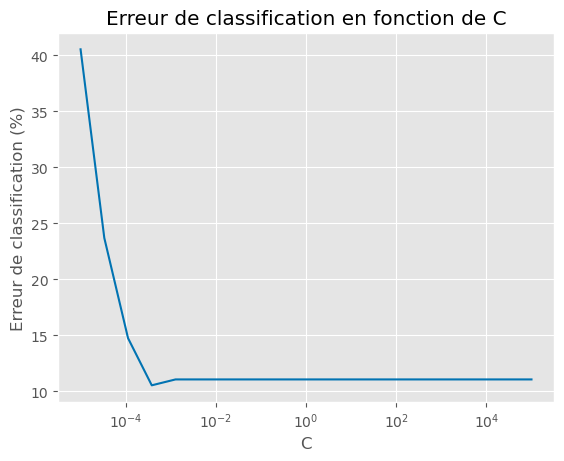
\includegraphics[width=0.65\linewidth]{images/erreur_C.png}}
\caption{Erreur de prédictions en fonction de C obtenue par validation croisée.}
\label{fig:err_C}
\end{figure}

On retrouve sur cette figure \ref{fig:err_C}, la valeur de $C=10^{-3}$ qui va minimiser l'erreur de prédiction.

\begin{lstlisting}
#courbe de l'erreur par cross validation
from sklearn.model_selection import cross_val_score
err = []

for C in Cs:
    clf = SVC(kernel='linear', C=C)
    scores = cross_val_score(clf, X_train, y_train, cv=5)
    err.append((1 - scores.mean())*100)
\end{lstlisting}

\newpage

Et qu'est ce que cela donne si on revient aux images ? 

\begin{figure}[H]
\centerline{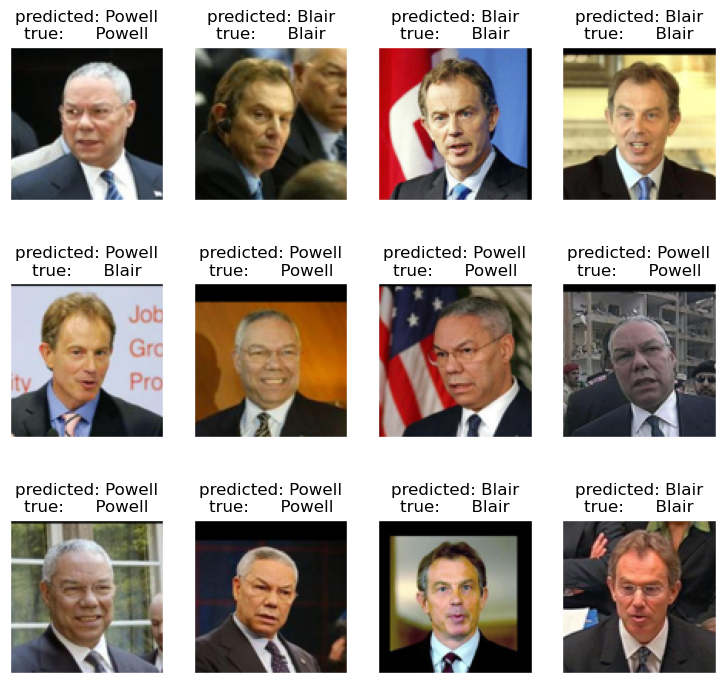
\includegraphics[width=0.8\linewidth]{images/pred_blair_powell.png}}
\caption{Prédiction entre Colin Powell et Tony Blair}
\label{fig:pow_blair}
\end{figure}

On observe en conséquence sur le jeu de données des images une erreur de une  prédiction sur les 12 ce qui correspond bien à une Accuracy de $0,91$.

\begin{figure}[H]
\centerline{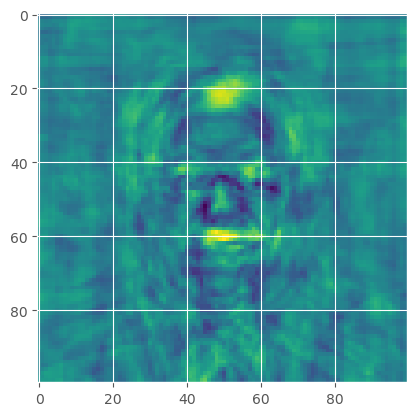
\includegraphics[width=0.5\linewidth]{images/coef_blair.png}}
\caption{Importance des différents pixels dans la décision}
\label{fig:pix_dec}
\end{figure}

Enfin sur la figure \ref{fig:pix_dec}, on peut apercevoir les pixels aux couleurs les plus intenses, claires ou foncées. Ce sont ces pixels, ces variables, qui apportent le plus de poids dans la prédiction de classification. 

\bigskip

\textbf{Question 5 : Introduction de nuisance}

J'ai décidé de fixer la graine à l'intérieur de la fonction \texttt{run\_svm\_cv}. Ainsi la comparaison se fera sur des jeux de données identiques. De plus dans la partie avec bruit, la ligne de code : 

\begin{lstlisting}
X_noisy = X_noisy[np.random.permutation(X.shape[0])]
\end{lstlisting}

n'est pas valable car on modifie les images mais pas les labels. De plus dans la fonction \texttt{run\_svm\_cv}, le mélange est déjà fait. Avec $\sigma=1$ on n'observe pas de différence et j'ai donc décidé d'augmenter sigma à $5$ qui est déjà une valeur importante car nos données sont déjà centrées et réduites.

\begin{lstlisting}
run_svm_cv(X,y)
run_svm_cv(X_noisy,y)
\end{lstlisting}

On observe donc une baisse du score. Il faudrait peut-être rajouter plus de variables de bruit pour observer une vraie baisse.

\begin{itemize}
\item[$\bullet$] Score sans variable de nuisance : 0.8947
\item[$\bullet$] Score avec variable de nuisance : 0.8158
\end{itemize} 

\bigskip

\textbf{Question 6 : score après réduction de dimensions}

En diminuant la dimension de l'espace de départ en cherchant les composantes principales par ACP voici les résultats obtenus :

\begin{table}[H]
\begin{center}
 \begin{tabular}{|l|*{6}{>{\centering\arraybackslash}p{2cm}|}}
\hline 
Nombre de composantes & 5 & 40 & 50 & 100  & 380 \\ 
\hline 
Score & 0.6105 & 0.9 & 0.8947 & 0.8842 &  0.8947   \\ 
\hline 
\end{tabular}
 \end{center} 
\caption{Score obtenu pour des variables bruitées en fonction du nombre de composantes principales}
\end{table}

\begin{lstlisting}
n_components = 40  # jouer avec ce parametre
print(f'Score apres reduction de dimension avec {n_components} composantes 
principales')
#on standardise pour pouvoir faire l'ACP
X_noisy_scale = StandardScaler().fit_transform(X_noisy)
pca = PCA(n_components=n_components,svd_solver='randomized')
X_pca = pca.fit_transform(X_noisy_scale)
run_svm_cv(X_pca,y)
\end{lstlisting}

On voit qu'en prenant un certain nombre de dimensions, on arrive à obtenir un meilleur score. Cela permet justement d'éliminer ce qui peut s'apparenter à du bruit qui aurait tendance à faire baisser le score.\\

Etrangement, avec 40 composantes principales, le score est supérieur au score sans variable de nuisance.\\

J'aurais aimé déterminer le score pour 10 et 20 composantes principales, mais le temps de calcul était trop long. 

\end{document}

